% =============================================================================
% Chapter 12 — Scaling Paths: Beyond the Pair
% =============================================================================

\chapter{Scaling Paths: Beyond the Pair}
\label{ch:scaling}

On this cluster, adding a third GPU makes long-context prefill
\emph{slower}: the repository's own warm A/B (2026-09-02) measured TTFT at 128k
and 256k running +22--23\,\% behind the two-node pair. That result is the
flavor of everything in this chapter. Every path out of the pair's limits
was actually measured, and none of them turned out to be a free win.

Everything before this chapter treated the two-Spark pair as the unit of
deployment: two GB10 boards, TP=2, one engine, one serving profile. But the
repository is honest about the pair's limits --- six decode slots, a KV pool
that supports roughly $2.3\times$ concurrency at the 1M context ceiling, and a
single point of failure. It explores every escape route an inference
engineer would reach for: a third node, a differently-built runtime image, a
second replica behind a router, shared weight storage, persistent KV, and a
genuinely 4-bit cache row. Each path carries a documented cost --- a
numerics hazard, an operational wedge, or a latency regression --- that the
repository states plainly. This chapter walks the six paths as considered
engineering trades, in roughly ascending order of how speculative they are.

For an inference engineer, this chapter is where scaling intuitions get
audited against a real system. ``Add a GPU'' silently assumes the work
shards; here MLA's replicated latent KV means it does not, and the honest
verdict is a capacity lane, not a speed lane. The same pattern --- a
plausible scaling move, a measurement, a cost the marketing version omits
--- repeats for every path below. The trade-offs (shard-layout
invariants, restart-order doctrines, allocator page arithmetic) are the
kind that transfer to any serving stack facing the same wall.

\section{A third Spark: TP=3}

The most literal scaling move is adding a third DGX Spark and running the same
model at tensor-parallel size~3. The repository supports it
(\repofile{docs/TP3.md} and \repofile{start-tp3.sh}) but frames it precisely: TP=3 is a
\emph{capacity} lane --- 16 slots, three times the KV --- not a speed lane.
The asymmetry behind that framing is worth carrying through the section: a
third rank divides the weight and MoE work, but MLA's latent KV and the
Lightning indexer are replicated on every rank, so the attention share of the
work does not shrink at all.

\subsection{The divisibility wall}

V4-Flash's attention geometry (\Cref{ch:model}) has
\code{num_attention_heads=64} arranged in 8 output groups, each feeding a
per-group BMM output projection. Tensor parallelism must divide the group
count: TP=2 splits 8 groups into 4 per rank cleanly, but 3 does not divide 8.
Stock vLLM handles this in the worst possible pair of ways. The config layer
refuses to start ($64 \,\%\, 3 \neq 0$); and if that check is bypassed, the
model code silently computes \code{8 // 3 == 2} local groups with no assert
--- six of the eight groups are simply dropped, and the engine serves fluent
garbage. A wrong shard that boots is far more dangerous than one that
crashes. The subtlest instance in this section is exactly that shape:
stock's \code{64 // 3 == 21} arithmetic produced \code{attn_sink} loader
windows of $[0{:}21][21{:}42][42{:}63]$, so head~63's sink weight was never
loaded on any rank. No assert, no crash, a healthy endpoint --- and a
silently wrong model.

The fix, vendored from localaiguyy's sister repository
\repofile{DeepSeek-V4-Flash-DSpark-3x-DGX-Spark}, pads the
geometry: groups $8 \to 9$, keeping heads-per-group at 8, so total heads
become 72 and each rank owns 3 groups and 24 heads. The entrypoint runs
\repofile{patches/tp3/apply_tp3_patch.py} inside the container only when
\envvar{TP_SIZE=3}; every edit is a no-op at TP$\le$2.

\subsection{Two generations of padding --- and the einsum that judges them}

The repository contains \emph{two} pad implementations that each declare the other
wrong, and the disagreement is the most instructive part of the story. The
question they disagree over has one deciding invariant, so state it first:
the checkpoint fixes the \code{o_proj} einsum's reduction dimension at
$r = \text{heads-per-group} \times \text{head\_dim} = 8 \times 512 = 4096$
--- the per-group output BMM contracts over $r$, and the \code{wo_a} slabs
are each $8192 \times 4096$. Any pad scheme is judged by whether its shard
layout preserves that contraction.

The top-level helper \repofile{patches/dsv4_tp_pad.py} implements resolution
R1: replicate all 8 groups on every rank and shard heads \emph{within} each
group, padding heads-per-group $8 \to 9$ so each rank takes 3 heads per
group. R1 was validated against the real fp8 checkpoint and reproduced TP=1
output at relative error $2.3\times10^{-6}$ --- fp8 quantization noise. It
keeps \code{wo_a}/\code{wo_b} \emph{replicated} (\code{disable_tp}), so
its local $r$ stays consistent with its own layout. The TP=3 patcher's
embedded module implements resolution R2: pad the \emph{group count}
$8 \to 9$ at constant heads-per-group, sharding \code{wo_a}/\code{wo_b}
normally on the padded group axis ($9216 \,\%\, 3 = 0$, 3072 rows per
rank). Its docstring declares R1 ``tried and STRUCTURALLY WRONG.''

Both are right --- about their own shard layout. Under R2's sharded layout,
only constant heads-per-group preserves $r=4096$: R1's 3~heads-per-group
would give $r=1536$ there, and DeepGEMM delivers the verdict by rejecting
the shape at \code{einsum.hpp:164}. The handbook lesson: a padding scheme
is only valid relative to a shard layout, and the kernel's contraction
contract --- not the divisibility arithmetic --- is the invariant that
decides (\Cref{fig:tp3-shard-layouts} lays the four candidate layouts over one
head axis).

\begin{figure}[htbp]
\centering
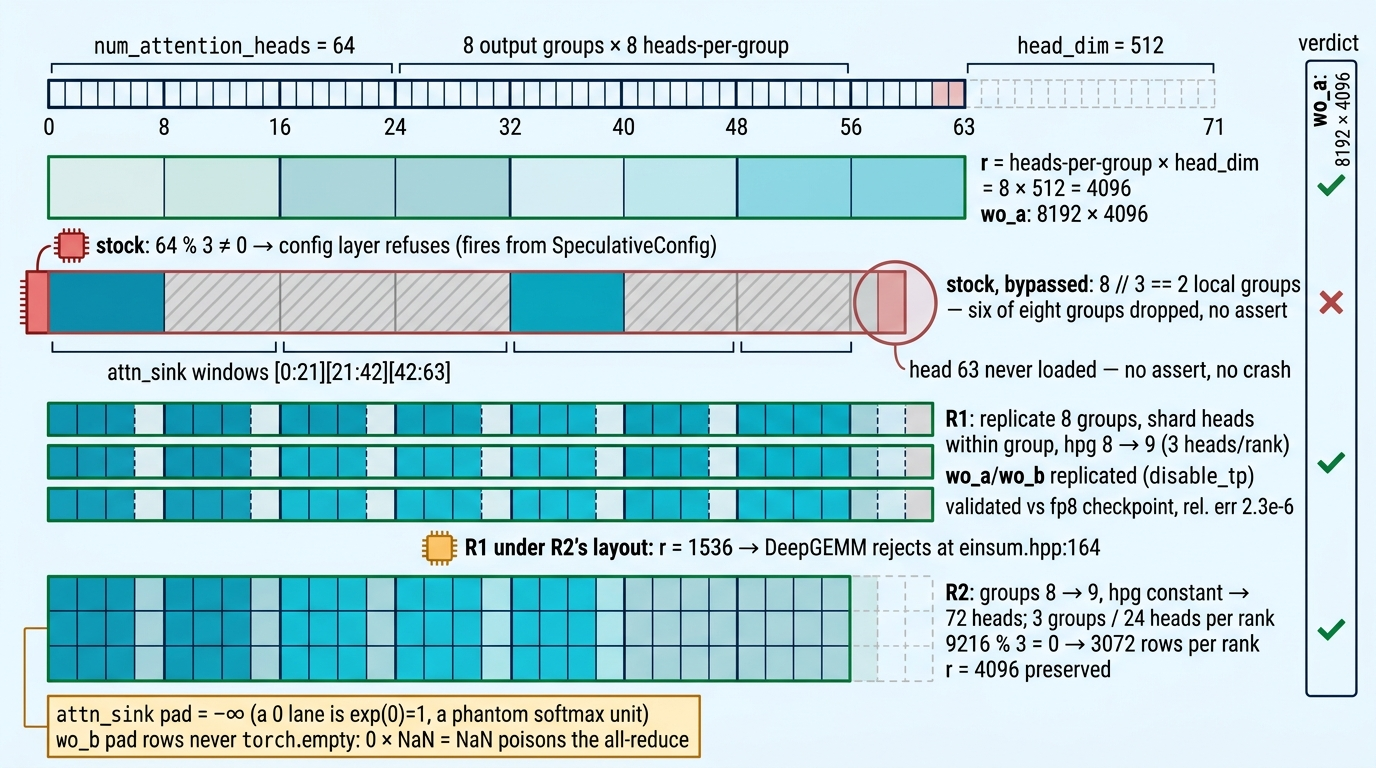
\includegraphics[width=\textwidth]{figures/ch12-shard-layouts.png}
\caption{Four ways to shard 64 heads across three ranks, judged by one
invariant. Stock refuses at the config layer ($64 \,\%\, 3 \neq 0$) and, if
bypassed, silently computes \code{8 // 3 == 2} local groups while its
\code{attn_sink} loader windows $[0{:}21][21{:}42][42{:}63]$ leave head~63
unloaded on every rank --- no assert, no crash, a healthy endpoint serving a
wrong model. R1 replicates the groups and shards heads within them, keeping
\code{wo_a}/\code{wo_b} replicated; it reproduces TP=1 output at
$2.3\times10^{-6}$ relative error under \emph{its own} layout, but its
3~heads-per-group would give $r = 1536$ under R2's sharded layout, which
DeepGEMM rejects at \code{einsum.hpp:164}. R2 pads the group count
$8 \to 9$ at constant heads-per-group, preserving the \code{o_proj}
contraction at $r = 4096$. A padding scheme is valid only relative to a
shard layout.}
\label{fig:tp3-shard-layouts}
\end{figure}

\begin{hblesson}
Pad lanes are not all equal. \repofile{dsv4_tp_pad.py}'s
\code{pad_fill_value} returns 0.0 for every parameter \emph{except}
\code{attn_sink}, which must be $-\infty$. The sink is an extra logit in the
softmax denominator: a zero pad lane contributes $\exp(0)=1$, a phantom unit
that attenuates every real attention weight --- ``plausible output, wrong
attention temperature.'' And \code{wo_b} pad rows must never be uninitialized
\code{torch.empty} memory, because $0 \times \mathrm{NaN} = \mathrm{NaN}$
poisons every rank through the all-reduce. Both TP-pad generations state this
independently; it is the most repeatable numerical-correctness lesson in the
patch corpus (\Cref{ch:patches}).
\end{hblesson}

The patcher applies eleven anchored edits, and their spread shows how deep a
``simple'' geometry change reaches. They include the config-layer
divisibility check (the actual boot blocker --- it fires from
\code{SpeculativeConfig} before any model class exists); three pad-aware
weight loaders in \repofile{parameter.py} that clamp the checkpoint copy to
what exists and zero-fill the tail --- with a documented replication trap
where offsetting a replicated parameter by \code{tp_rank} would silently
zero it on ranks $\ge 1$; MoE intermediate size $2048 \to 2112$ (a multiple
of $\mathrm{lcm}(3,64)=192$, so each rank's 704 columns stay 64-aligned for
NVFP4); vocab padding $129{,}280 \to 129{,}408$;
and the \code{attn_sink} loader windows that fix the silent head-63 drop
above.

\begin{hbwarstory}
The TP=3 patcher's idempotence markers originally hashed the patch
\emph{description}. When the patch body changed, a container whose writable
layer held the old patched file still looked ``already patched'' --- and that
layer survives every \code{docker compose restart} (restart is not recreate).
The only symptom was a shape assert on rank~2. The patcher now embeds a
SHA-256 prefix of the replacement body in each marker. A stale body yields
\code{STALE}, a hard exit-1 whose remediation is explicit: \code{docker rm -f}
on every node, because the anchor text was consumed and the file cannot be
re-anchored in place. \code{MISS} is equally fatal --- ``an unpatched
attn\_sink loader fails SILENTLY.''
\end{hbwarstory}

\subsection{One launcher per topology}

Three Sparks get a separate launcher, \repofile{start-tp3.sh}, and the reason
is stated in \repofile{docs/TP3.md}: a \envvar{TP_SIZE=3} line in
\repofile{.env.dspark} must not be able to silently change the two-node path.
The wrapper requires both \envvar{WORKER_HOST} and \envvar{WORKER2_HOST},
hard-fails if the patch file is missing, exports \envvar{DSPARK_TP3=1},
\envvar{TP_SIZE=3}, \envvar{NNODES=3}, and \code{exec}s the standard
launcher. Concurrency is likewise namespaced: \envvar{TP3_MAX_NUM_SEQS}
(or \code{--max-num-seqs 16}) is honored only by the TP=3 wrapper and ignored
by the two-node start, so an experiment's knobs cannot leak into the
production lane. One detail is quietly ahead of its sibling: the TP=3 usage
text documents CUDA-graph capture size as
$N \times (\text{MTP\_NUM\_TOKENS}+1)$ \emph{rounded up to a multiple of 8}
--- exactly the rounding whose absence on the TP=2 lane left the $c{=}6$
decode shape uncaptured (\Cref{ch:perf}).

\subsection{Bootstrapping the ring}

On a QSFP ring the third Spark is not on the spark1$\leftrightarrow$spark2
subnet: each pairwise link carries its own /24 (head
\code{10.0.22.1}$\,\leftrightarrow\,$\code{10.0.22.2} to spark2;
\code{10.0.23.1}$\,\leftrightarrow\,$\code{10.0.23.3} to spark3). That breaks
three assumptions the two-node fabric setup (\Cref{ch:fabric}) never had to
question, and the launcher rewires all three:

\begin{itemize}
\item \textbf{Bootstrap moves to the LAN.} Gloo, the NCCL socket, and the TP
TCP store move onto \envvar{TP3_BOOTSTRAP_IFNAME} (default \code{enP7s7})
--- the one network all three nodes share, and never \code{lo}, where Gloo
binds \code{127.0.0.1} and the mesh fails.
\item \textbf{Both head HCAs.} \envvar{NCCL_IB_HCA} is set to
\code{rocep1s0f0,rocep1s0f1} so spark1 faces both links (a single facing
HCA times out in QP RTR). And spark3's \envvar{WORKER2_NCCL_*} must be
pinned to its own port facing spark1, not copied from
\envvar{WORKER_NCCL_*}.
\item \textbf{Subnet-aware GID pairing.} The launcher disables NIC merging
(\envvar{NCCL_IB_MERGE_NICS=0}), enables subnet-aware routing, and sets
\envvar{NCCL_IB_SUBNET_PREFIX_LEN=24}: the default /16 would treat both /24s
as one subnet and pair GIDs across links that cannot reach each other.
\end{itemize}

\needspace{9\baselineskip}
\begin{lstlisting}[language=bash]
# .env.dspark additions for the third Spark (docs/TP3.md)
WORKER2_HOST=10.0.0.3
WORKER2_VLLM_HOST_IP=10.0.0.3
WORKER2_NFS_SERVER_IP=10.0.23.1   # head IP on the spark1<->spark3 link
WORKER2_NCCL_IB_HCA=rocep1s0f1    # spark3's port FACING the head
WORKER2_NCCL_SOCKET_IFNAME=enp1s0f1np1
WORKER2_TP_SOCKET_IFNAME=enp1s0f1np1
WORKER2_GLOO_SOCKET_IFNAME=enp1s0f1np1

./prepare-dspark-model-cache.sh --yes
./start-tp3.sh --max-num-seqs 16
scripts/validate_tp3.sh 127.0.0.1:8888   # prove the shard, not just HTTP
\end{lstlisting}

\begin{figure}[htbp]
\centering
\begin{tikzpicture}[node distance=10mm and 14mm]
  % nodes
  \node[hbhost, minimum width=34mm] (s1)
    {\textbf{spark1 (head)}\\rank 0 \(\cdot\) NFS exporter\\rocep1s0f0 + rocep1s0f1};
  \node[hbhost, below left=16mm and 8mm of s1, minimum width=30mm] (s2)
    {\textbf{spark2}\\rank 1\\mounts 10.0.22.1};
  \node[hbhost, below right=16mm and 8mm of s1, minimum width=30mm] (s3)
    {\textbf{spark3}\\rank 2\\mounts 10.0.23.1};
  % QSFP links
  \draw[hbarrow, <->, very thick] (s1.south west) -- (s2.north)
    node[hblabel, midway, left=2mm, align=right] {QSFP\\10.0.22.0/24};
  \draw[hbarrow, <->, very thick] (s1.south east) -- (s3.north)
    node[hblabel, midway, right=2mm, align=left] {QSFP\\10.0.23.0/24};
  \draw[hbarrow, <->, dashed, color=hbSteel!60] (s2.east) -- (s3.west)
    node[hblabel, pos=0.25, above=1mm, fill=white, inner sep=1pt] {ring segment};
  % NFS flows
  \draw[hbflow, bend right=28] (s1.west) to
    node[hblabel, above left=0mm and 1mm] {NFS ro} (s2.north west);
  \draw[hbflow, bend left=28] (s1.east) to
    node[hblabel, above right=0mm and 1mm] {NFS ro} (s3.north east);
  % LAN bus
  \coordinate (lanl) at ($(s2.south)+(-6mm,-9mm)$);
  \coordinate (lanr) at ($(s3.south)+(6mm,-9mm)$);
  \draw[very thick, color=hbGreen!70!black] (lanl) -- (lanr)
    node[hblabel, midway, below=1mm, color=hbGreen!70!black]
    {LAN enP7s7 \(\cdot\) 192.168.1.0/24 --- Gloo bootstrap, NCCL socket, TP TCP};
  \draw[hbok] (s2.south) -- ($(s2.south)+(0,-9mm)$);
  \draw[hbok] (s3.south) -- ($(s3.south)+(0,-9mm)$);
  \draw[hbok] (s1.south) .. controls +(0,-14mm) and +(0,10mm) ..
    ($(lanl)!0.5!(lanr)$);
  % NCCL knob annotation
  \node[hbpatch, right=6mm of s1, align=left, font=\scriptsize] (knobs)
    {NCCL\_IB\_MERGE\_NICS=0\\NCCL\_IB\_SUBNET\_AWARE\_ROUTING=1\\NCCL\_IB\_SUBNET\_PREFIX\_LEN=24};
  \draw[hbarrow, dashed] (knobs.west) -- (s1.east);
\end{tikzpicture}
\caption{TP=3 on the QSFP ring. Each pairwise link is its own /24, so NCCL
needs both head HCAs and /24-aware GID pairing; process-group bootstrap rides
the shared LAN, never \code{lo}. Worker~2 mounts the head's HF cache at the
head's address \emph{on its own link} (10.0.23.1), which the start script
grants to the live NFS exporter.}
\label{fig:tp3-ring}
\end{figure}

The launcher checks --- but does not perform --- the third node's
prerequisites: passwordless SSH, and the pinned $\approx$19\,GB vLLM image
already pulled (it refuses to boot and prints the exact \code{docker pull}
command otherwise). With \envvar{DSPARK_WORKER_HF_NFS=1} it syncs compose,
env, and \repofile{patches/tp3/}, and mounts the head's HF cache over NFS, so
spark3 needs no local checkpoint.

\subsection{What three nodes buy --- and what they cost}

\Cref{tab:tp3-ledger} is the repository's own warm A/B (2026-09-02, same image,
prose prompts, 512 output tokens; TP=3 at 16 slots vs TP=2 at 6).

\begin{table}[htbp]
\centering\small
\caption{The TP=3 ledger (\repofile{docs/TP3.md}, reference cluster).}
\label{tab:tp3-ledger}
\begin{tabular}{lll}
\toprule
Load & TP=2 & TP=3 \\
\midrule
decode, 1 stream & 38.6 \tokspersec{} & 41.9 \tokspersec{} (+9\,\%) \\
decode, 2 streams & 63.9 agg & 72.0 agg (+13\,\%) \\
decode, 4 streams & 86.0 agg & 89.7 agg (+4\,\%) \\
decode, 8 / 12 / 16 streams & n/a (6 slots) & 142.8 / 164.3 / 198.0 agg \\
TTFT 8k / 16k / 32k / 64k & 4.4 / 8.7 / 18.0 / 36.0 s & +4--13\,\% slower \\
TTFT 128k / 256k & 74.9 / 164.8 s & 91.5 / 202.2 s (+22--23\,\%) \\
KV cache per rank & $\approx$16.8 / 15\,GiB & $\approx$35 / 34 / 35\,GiB \\
\bottomrule
\end{tabular}
\end{table}

The headline: 16 slots, $\approx$5.0M KV tokens ($4.8\times$ concurrency at
1M), $\approx$200 \tokspersec{} aggregate at $c{=}16$, and modestly faster
per-stream decode (+4--13\,\%) --- against prefill that is 4--23\,\%
\emph{slower}, worst at $\ge$128k. The ``why'' is architectural, not
incidental. In DeepSeek's MLA every rank holds the full latent KV and the
Lightning indexer is replicated (\Cref{ch:architecture}), so the attention
share of prefill does not shrink with a third GPU. Meanwhile the pad (heads
$64 \to 72$) adds real work, and a three-rank ring all-reduce over two
different physical links costs roughly twice the latency of a two-rank
exchange.

The audit's first-principles model (\Cref{ch:perf}) makes the same
point from the decode side: bytes per rank per step drop from
$\approx$16.5\,GB to $\approx$11.5\,GB, yet the measured step barely
moves.
Bandwidth arithmetic alone predicts a $\approx$48\,ms step from those
11.5\,GB; the measured step is $\approx$61\,ms --- roughly 13\,ms of fixed
per-step cost, and the bandwidth gain is gone. That single measurement is
the mechanism behind the chapter's opening headline: the fixed overheads a
third rank adds --- a three-rank ring over two different physical links,
the padded heads' extra work --- are exactly what the unshrinkable
attention share of prefill pays at 128k--256k, surfacing as the +22\,\%
TTFT regression. TP=3 is a capacity trade; single-user long-context work
stays on the two-node lane.

\begin{hbnote}
First boot at TP=3 is slow by design, not broken. Spark3 starts with an empty
JIT cache and the TP=3 shard shapes are new for all three nodes, so the first
\repofile{start-tp3.sh} spends several minutes compiling ($\approx$8 minutes
to healthy on the reference pair; engine init alone 193\,s). The first
requests still hit Triton JIT spikes. Do not restart a boot that is merely
compiling --- wait for \code{HEALTH_OK} / \code{boot-shape-warmup}. Later
boots reuse the persisted caches.
\end{hbnote}

\section{The Stage-C lane: 200K $\times$ 16}

The second scaling path changes the \emph{runtime}, not the node count. The
default serve lane patches the pinned Anemll image at container start
(\Cref{ch:patches}). The \repofile{recipe/} lineage instead bakes the
$\approx$20 DSpark overlay source files over a different base ---
\repofile{ghcr.io/bjk110/vllm-spark:unholy-fusion-prod-ready}, the
``unholy fusion'' GB10 build carrying the B12X MoE kernels --- with a
\code{py_compile} gate at build time. On top of that clean overlay sit three
NVFP4 stages whose names tell the story of a probe and a retreat:

\begin{description}
\item[Stage A --- the dtype exists.] Registers \code{nvfp4_ds_mla} in
\code{CacheDType}, maps it to \code{torch.uint8} and
\code{KVQuantMode.NVFP4}, and gives the KV interface a real-page-size branch
at 416 bytes per token.
\item[Stage B --- the 416\,B probe.] Teaches the DeepSeek-V4 attention layer
to accept the dtype with \code{head_bytes = 416} --- the GLM-5.2 NVFP4
sparse-MLA per-token record --- to probe whether DSV4's store/decode kernels
are compatible with the GLM record. They are not, yet.
\item[Stage C --- retreat to the known envelope.] \sloppy Rewrites the
416-byte cells back to DeepSeek V4's proven \textbf{584-byte} envelope for
\code{nvfp4_ds_mla}, model-version-gated. The in-line rationale: keep the
hybrid MLA/SWA grouping bootable first (``padded NVFP4 probe''); kernel and
store correctness is the next experiment.
\end{description}

Stage C is where the \envvar{VLLM_DSPARK_*} tuning family actually exists.
On the Anemll 0.1.1 image those keys are unregistered and produce only
``Unknown vLLM environment variable'' warnings ---
\repofile{docker-compose.stage-c.override.yml} is inert there by design. The
one that matters most for scale is
\envvar{VLLM_DSPARK_GPU_REJECTED_CONTEXT_MASK=1}, the ragged-batch path
required once the Keys concurrency patch (request-stable draft-KV slots,
\Cref{ch:specdecode}) unlocks \code{max_num_seqs > 1} with mixed
prefill+decode batches.

The measured lane --- Stage-C image, \code{max_model_len=200000},
\code{max_num_seqs=16}, Keys patch at \code{7e4d94bb} --- is summarized in
\Cref{tab:stagec-lane}.

\begin{table}[htbp]
\centering\small
\caption{The Stage-C lane, measured (aggregate \tokspersec{}; per-stream and
acceptance in parentheses).}
\label{tab:stagec-lane}
\begin{tabular}{@{}llll@{}}
\toprule
Arrivals & $c{=}1$ & $c{=}8$ & $c{=}16$ \\
\midrule
static & 57.6 (acc.\ 0.635) & 252.6 (31.6/stream) &
\textbf{315.1} (19.7/stream, 0.609) \\
staggered & --- & --- & 205.0 \\
\bottomrule
\end{tabular}
\end{table}

The repository's own caveat deserves
repeating verbatim in spirit: this is a \emph{short-context, high-aggregate}
profile --- a different product than the 1M-context agent lane, not a faster
version of it.

\section{Horizontal scale-out: replicas behind a router}

Both paths so far change the engine --- its shard geometry or its runtime
image. The least glamorous path changes neither, and it is the one
\repofile{docs/SETUP.md} actually ran:
four Sparks as \emph{two independent TP=2 replicas} serving the same
DeepSeek-V4-Flash-DSpark checkpoint. Replica A was the control --- the
Rafael Caricio stack, unpatched, pinned at \code{max-num-seqs=1}, holding
$\approx$52--54 \tokspersec{} single-stream throughout. Replica B ran the
packaged recipe with the Keys concurrency patch and swept
\code{max-num-seqs} from 1 to 16, so every concurrency claim in the recipe
was measured against a live unpatched baseline on identical hardware,
serving at the same time. The experiment's shape is as instructive as its
numbers: nothing about a second pair required new numerics, new fabric
work, or a new launcher --- replica B could be patched, swept, and rolled
back while replica A kept serving.

That layout generalizes into SETUP.md's final step: run a second patched
TP=2 replica and put a least-connections router in front for roughly
$2\times$ aggregate throughput and concurrency. Because replicas share
nothing at runtime, this path has none of TP=3's numerics or fabric risk
--- and none of its KV-pool consolidation either. Each replica keeps its
own $\approx$2.3M-token pool, and a request sees only its replica's cache.
Where the workload is many independent sessions rather than one giant
context, the router is the better trade (\Cref{fig:kv-two-ways} draws the
three capacity paths against what a single request can actually reach); the
two lanes compose, since each replica could itself be a TP=3 triple.

\begin{figure}[htbp]
\centering
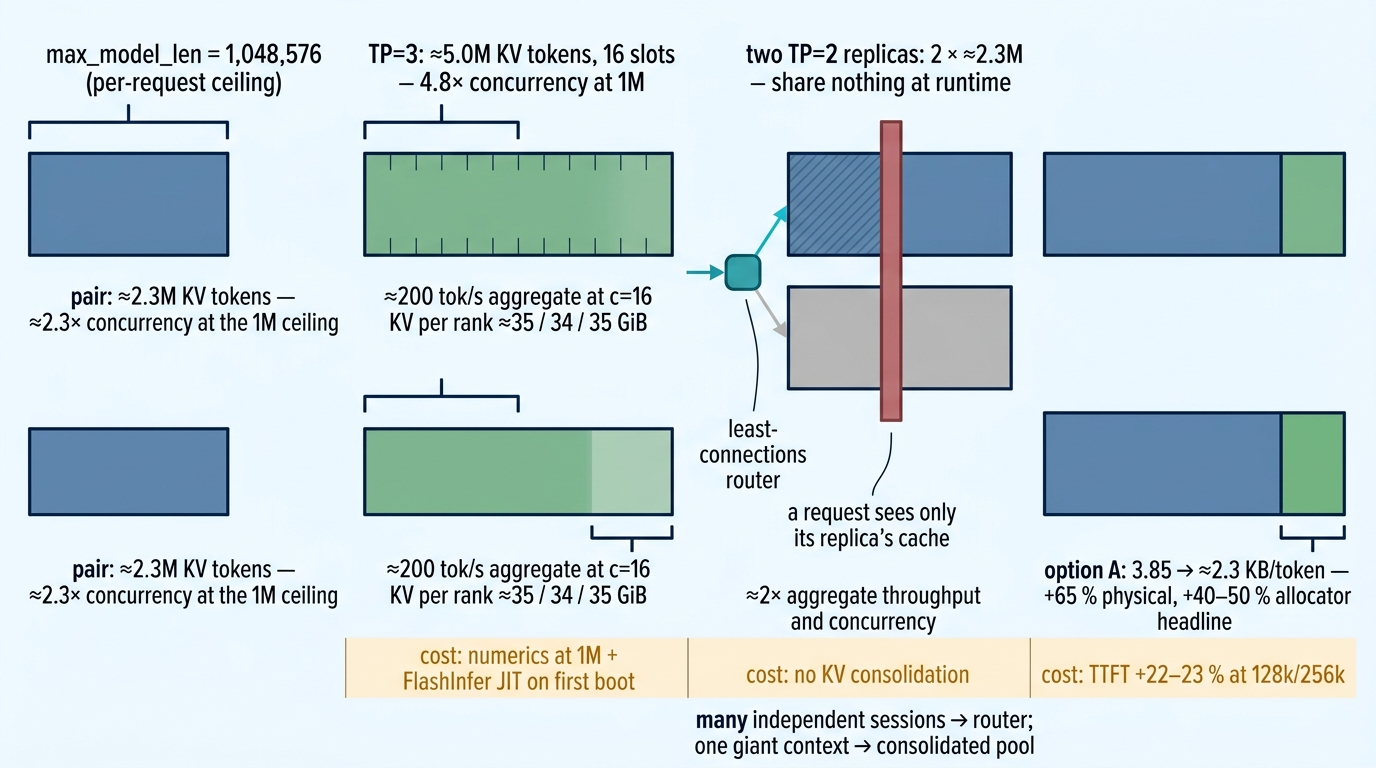
\includegraphics[width=\textwidth]{figures/ch12-two-ways-kv.png}
\caption{More KV is not one thing. TP=3 consolidates into a single
$\approx$5.0M-token pool ($4.8\times$ concurrency at the 1M ceiling, 16
slots) that one request can draw from --- paid for with prefill 4--23\,\%
slower and TTFT +22--23\,\% at 128k--256k. Two TP=2 replicas behind a
least-connections router give $\approx 2\times$ aggregate throughput with
none of TP=3's numerics or fabric risk, but they share nothing at runtime:
each keeps its own $\approx$2.3M-token pool and a request sees only its
replica's cache. Item-8's option-A row grows the existing pool in place
instead, $\approx$3.85 $\to$ $\approx$2.3\,KB per token. The lanes compose
--- each replica could itself be a TP=3 triple.}
\label{fig:kv-two-ways}
\end{figure}

\section{Weights logistics at scale}

Every extra node multiplies a mundane problem: the checkpoint is hundreds of
gigabytes, and the abliterated variant nearly doubles it if copied naively.

\subsection{NFS mode: one copy of the weights}

With \envvar{DSPARK_WORKER_HF_NFS=1}, workers keep no local checkpoint. The
head exports its HuggingFace cache read-only over the ConnectX fabric from a
privileged Alpine container running a \emph{kernel} NFSv4-only server
(\repofile{files/nfs-server/}): the entrypoint mounts \code{nfsd} and
\code{rpc_pipefs}, generates \repofile{/etc/exports} with one line per
client, then runs \code{rpc.nfsd 8}. Two design points carry the operational
weight:

\begin{itemize}
\item \textbf{Live-exporter reuse.} \code{nfs_ensure_server} first probes
\code{rpcinfo -t $ip nfs 4}; if \emph{any} NFSv4 server already answers
(the Qwen recipe's \code{vllm-fn-nfs}, or a previous \code{dspark-nfs}), it
is reused rather than duplicated. The comment explains why: kernel nfsd in a
privileged container can leave rpcbind in D-state, and then
\code{docker rm -f} hangs --- ``do not docker rm a working share.'' For the
third node, \code{nfs_grant_subnet} appends the new /24 to the \emph{running}
exporter's exports and re-runs \code{exportfs -rav}, without recreating a
container another recipe may be using. Teardown
(\repofile{stop-deepseek-v4-flash-dspark.sh}~\code{--nfs}) removes only the
DSpark-owned exporter, never \code{vllm-fn-nfs}.
\item \textbf{Read-only weights, writable JIT.} The worker mounts the named
volume \code{dspark-hf} (\code{nfsvers=4.2,ro,nconnect=8}, 1\,MiB
rsize/wsize, \code{hard,timeo=600}) in place of the host HF bind. The
override compose overlays \emph{six local writable bind mounts} on top of the
read-only tree --- \code{triton-cache}, \code{tilelang-cache},
\code{vllm-cache}, \code{flashinfer}, \code{b12x-cute-cache},
\code{nccl-fr}. Compiled-kernel caches must be per-node and writable while
weights stream read-only from one copy; the head pre-creates the mount-point
directories because overlay points must already exist on a read-only export.
\end{itemize}

\subsection{The 26-shard abliterated overlay}
\label{sec:scale-ablit-overlay}

The abliterated Vision-Exp variant edits only layers 10--35
\code{attn.wo_b} --- 26 tensors packed in shards 00012--00037.
\repofile{scripts/overlay-vision-exp-ablit-cache.py} exploits that:
it classifies blobs shared between the official and abliterated snapshots,
\emph{hardlinks} the shared ones into the abliterated repository's blob store,
copies (or rsyncs to the worker, via a \code{--files-from} list) only the
unique shards, and rebuilds the snapshot symlink tree. A manifest mode
exports the classification as JSON so a node without the source cache can
verify ``unique ablit blobs missing ($N$)'' and fail with the list. Two
near-identical multi-hundred-GB models cost one checkpoint plus 26 shards.

\section{KV persistence: LMCache}

Shared storage settles where the weights live; it does nothing for the
other large state a restart destroys. Restarting the engine normally
forfeits every cached context; at 1M-class
contexts that is minutes of re-prefill per session. The experimental
\repofile{lmcache/} option keeps KV in per-node \code{lmcache server}
processes (L1 in CPU RAM, filesystem L2 on local NVMe) that survive engine
restarts, wired in through \code{LMCacheMPConnector} over ZMQ on the fabric
IPs. The measured win is dramatic: a $\approx$107K-token context that costs
$\approx$65\,s to re-prefill reloads in \textbf{1.8--1.9\,s} (measured
$n{=}2$, GB10 pair, \code{nvfp4_ds_mla}). What that reload costs is
structural rather than numerical: the KV outlives the engine precisely
because it now lives in a process the engine's own lifecycle does not own,
and each failure mode below follows from that single fact.

The README then spends most of its length on why you might \emph{not} turn it
on, under an explicit ``owner decision required'' heading. Three named
failure modes:

\begin{enumerate}
\item \textbf{The servers live outside Compose.} They are plain
\code{docker run} containers --- not started, stopped, health-checked, or
supervised with the model containers --- and the stop script
(\repofile{stop-deepseek-v4-flash-dspark.sh}) leaves them running. Boot order
is manual and load-bearing: every node's server must be up \emph{and
verified} before the engine starts.
\item \textbf{Confirmed unified-memory cold-boot OOM.} On 128\,GB
unified-memory boards the kernel OOM killer has killed the server during an
engine cold boot --- the weight-load spike lands on top of the server's
resident L1 (confirmed in \code{dmesg}; reported upstream as LMCache \#4759).
Mitigations: size L1 down, and optionally set \envvar{LMCACHE_OOM_SCORE_ADJ}
negative so the killer prefers the Compose-restarted engine over the
unsupervised server. The recipe deliberately defaults that knob to 0,
because it is a node-wide policy choice ``not ours to make.''
\item \textbf{A dead server wedges the engine --- silently.} A restarted or
killed server loses its GPU contexts; current upstream code then parks every
lookup-hit request forever. The scheduler heartbeat never starts, so dead
servers stay ``healthy''; lookup errors do not propagate; the engine neither
crashes nor falls back to re-prefill. An operator watching container exits
sees a healthy pair serving nothing.
\end{enumerate}

\begin{hbwarning}
Failure mode 3 dictates the restart-order doctrine. Servers run with
\code{--restart no} --- a dead server must stay dead and \emph{visible}.
The launcher refuses to recreate a server while any \code{vllm-dspark}
container is live, because a fresh server under a live engine \emph{is} the
wedge. The only supported recovery is a full-pair restart, servers first,
then the engine. Moving the servers into Compose is deliberately out of
scope: Compose auto-restarting an emptied server is exactly the wedge. Until
LMCache PR \#4764 (heartbeat) lands, the blast radius of a dead cache server
is the model service.
\end{hbwarning}

Two configuration invariants are non-negotiable: \envvar{PYTHONHASHSEED=0} on
every process (chunk keys use Python's randomized \code{hash()}; unpinned,
every restart invalidates the whole cache --- LMCache \#1788), and L1 sized
to the largest context (\code{--l1-size-gb 12} for $\approx$150K-token
documents; mid-store L1 eviction has stalled stores). The compose patcher
puts every LMCache delta inside one entrypoint branch gated on
\envvar{DSPARK_ENABLE_LMCACHE} being exactly \code{1}, so a single compose
file serves both modes and the off state is verifiably stock.

\begin{lstlisting}[language=bash]
# one server per node, bound to THAT node's fabric IP; both must verify
./lmcache/run-lmcache-server.sh 192.168.104.10   # head
./lmcache/run-lmcache-server.sh 192.168.104.11   # worker
python3 lmcache/patch-compose-lmcache.py \
  docker-compose.dspark.yml docker-compose.lmcache.yml \
  tcp://192.168.104.10:6667,tcp://192.168.104.11:6667
export DSPARK_ENABLE_LMCACHE=1
COMPOSE_FILE=$PWD/docker-compose.lmcache.yml ./start-deepseek-v4-flash-dspark.sh
\end{lstlisting}

\begin{figure}[htbp]
\centering
\adjustbox{max width=\textwidth}{%
\begin{tikzpicture}[node distance=6mm and 10mm]
  % head node group
  \node[hbgpu, minimum width=30mm] (eng) {vLLM engine\\(vllm-dspark, rank 0)};
  \node[hbnode, right=34mm of eng, minimum width=30mm] (srv)
    {lmcache server\\L1: 12\,GB CPU RAM};
  \node[hbhost, below=of srv, minimum width=30mm] (l2) {L2: local NVMe\\(fs adapter)};
  \node[hbfaint, below=of eng, minimum width=30mm] (worker)
    {worker node:\\same pair, mirrored};
  \begin{scope}[on background layer]
    \node[hbgroup, fit=(eng)(worker), label={[hbtitle]above:Compose lifecycle}] (grp) {};
  \end{scope}
  \draw[hbflow, <->] (eng) -- (srv)
    node[hblabel, pos=0.55, above=0.5mm, font=\tiny] {ZMQ tcp://fabric-ip:6667};
  \draw[hbarrow, <->] (srv) -- (l2);
  % failure-mode annotations
  \node[hbwarn, right=12mm of srv, align=left, font=\scriptsize] (f1)
    {F1: outside Compose ---\\manual, load-bearing\\boot order};
  \node[hbwarn, below=4mm of f1, align=left, font=\scriptsize] (f2)
    {F2: cold-boot OOM ---\\weight-load spike +\\resident L1 (dmesg)};
  \node[hbwarn, below=4mm of f2, align=left, font=\scriptsize] (f3)
    {F3: dead server parks\\lookup hits forever ---\\engine wedges silently};
  \draw[hbfail] (f1.west) -- (srv.north east);
  \draw[hbfail] (f2.west) -- (srv.east);
  \draw[hbfail] (f3.south) to[bend left=25] (worker.east);
  % doctrine
  \node[hblabel, below=4mm of worker, align=center]
    {-{}-restart no \(\cdot\) servers up before engine \(\cdot\)\\
     recovery = full-pair restart, servers first};
\end{tikzpicture}%
}
\caption{LMCache on the pair: per-node cache servers outside the Compose
lifecycle, ZMQ on the fabric IPs, L1 RAM + L2 NVMe. The three named failure
modes (red) are why enabling it is framed as an owner decision, not a free
$65\,\mathrm{s} \to 1.9\,\mathrm{s}$ win.}
\label{fig:lmcache-arch}
\end{figure}

\section{The 4-bit KV future}

LMCache stretches the KV pool across restarts; the last path stretches it
in place, and it is the deepest: making the cache row actually 4-bit. It is
also the path whose binding constraint sits somewhere other than intuition
puts it --- not how few bits attention can tolerate, but which row sizes the
hybrid KV allocator's uniform page will accept --- so the arithmetic that
follows is a search for a divisor as much as for a precision. Today
\code{nvfp4_ds_mla} is byte-identical to \code{fp8_ds_mla} --- 584 bytes per
token: 448\,B of fp8 e4m3 NoPE with seven UE8M0 per-64 scales, 128\,B of
bf16 RoPE, and an 8-byte footer. The ``nvfp4'' string changes only kernel
dispatch (which is why issue \ghissue{22} routed it to the fp8 kernel).
\repofile{docs/CLAUDE/item8-fp4-kv-design.md} is the design study for a real
compressed row. Its central constraint comes from vLLM's hybrid KV
allocator: every KV group --- 1 MLA plus 3 sliding-window groups --- must
share the same page size in bytes, today $64 \times 584 = 37{,}376$\,B. Only
row sizes that divide that page with a power-of-two row count are cheap:
$584 \times 64 = 292 \times 128 = 146 \times 256$. That arithmetic sorts the
options (\Cref{tab:fp4-options}).

\begin{table}[htbp]
\centering\footnotesize
\caption{Item-8 layout options for the compressed (C4/C128) row against the
uniform-page constraint.}
\label{tab:fp4-options}
\begin{tabular}{>{\raggedright\arraybackslash}p{2.6cm}>{\raggedright\arraybackslash}p{3.6cm}p{1.4cm}p{1.3cm}>{\raggedright\arraybackslash}p{3.4cm}}
\toprule
Option & Row & Bytes & Fits page? & Risk / cost \\
\midrule
A --- half row & e2m1 NoPE + 4 UE8M0 scales per 128 + fp8 RoPE &
292 & yes (exact) & block-128 scaling coarse for e2m1; one quant-tile change \\
B --- fp4 RoPE & MXFP4 NoPE (per-32) + e2m1 RoPE & 280/292 & yes &
positional precision at 1M --- highest quality risk \\
C --- keep bf16 RoPE & 224 + 14 + 128\,B RoPE & 366$\to$368 & \textbf{no} &
needs per-group page sizes (upstream allocator change); SWA row is written by
a C++ op \\
D --- DCP-2, no fp4 & keep 584\,B; shard \emph{tokens} across ranks & --- &
n/a & zero numerics risk; DSV4 sparse backend has no DCP in this image \\
\bottomrule
\end{tabular}
\end{table}

The recommendation is to prototype \textbf{option A} first: it fits the page
exactly at 292 bytes, preserves RoPE at fp8, and changes one quantization
tile. Expected capacity: the compressed per-token term drops from 3.07 to
1.54\,KB, total physical bytes from $\approx$3.85 to $\approx$2.3\,KB/token
--- \textbf{+65\,\% tokens at the physical level}, +40--50\,\% in the
allocator headline (the SWA groups keep 584-byte pages). The study is candid
that the headline ``2.33M tokens in 17.04\,GiB'' is allocator accounting
across four groups, not physical row cost --- which is exactly why shrinking
the compressed row moves capacity more than linearly.

\begin{figure}[htbp]
\centering
\begin{tikzpicture}
  % scale: 0.021 cm per byte
  % Row 1: 584 B  (448 | 128 | 8)
  \node[hbtitle, anchor=south west] at (0,1.05) {today: 584 B/token
    (\,fp8\_ds\_mla \(=\) nvfp4\_ds\_mla\,)};
  \draw[fill=hbBlue!10, draw=hbSteel, thick] (0,0) rectangle (9.41,0.9);
  \node[font=\scriptsize] at (4.7,0.45)
    {NoPE 448 B --- fp8 e4m3, 7 UE8M0 scales per 64 dims};
  \draw[fill=hbGreen!12, draw=hbSteel, thick] (9.41,0) rectangle (12.10,0.9);
  \node[font=\scriptsize, align=center] at (10.75,0.45) {RoPE 128 B\\(64 \(\times\) bf16)};
  \draw[fill=hbAmber!35, draw=hbSteel, thick] (12.10,0) rectangle (12.27,0.9);
  \node[hblabel, anchor=north east, font=\tiny] (foot) at (12.27,-0.12) {footer 8 B (7 scales + pad)};
  \draw[hbarrow] (foot.north) -- (12.18,-0.02);
  % Row 2: 292 B  (224 | 4 | 64)
  \node[hbtitle, anchor=south west] at (0,-1.35) {option A: 292 B/token
    (proposed nvfp4c\_ds\_mla)};
  \draw[fill=hbBlue!10, draw=hbSteel, thick] (0,-2.4) rectangle (4.70,-1.5);
  \node[font=\scriptsize] at (2.35,-1.95) {NoPE 224 B --- e2m1 (2/byte)};
  \draw[fill=hbAmber!35, draw=hbSteel, thick] (4.70,-2.4) rectangle (4.79,-1.5);
  \draw[fill=hbGreen!12, draw=hbSteel, thick] (4.79,-2.4) rectangle (6.13,-1.5);
  \node[hblabel, anchor=west] (sc) at (6.6,-1.7) {4 \(\times\) UE8M0 per-128 (4 B)};
  \draw[hbarrow] (sc.west) -- (4.745,-1.52);
  \node[hblabel, anchor=west] (rp) at (6.6,-2.15) {RoPE 64 B (fp8)};
  \draw[hbarrow] (rp.west) -- (6.13,-1.95);
  % page arithmetic
  \node[hblabel, anchor=north west, align=left] at (0,-2.8)
    {same 37{,}376-byte page: 64 rows \(\times\) 584 B \(=\) 128 rows
     \(\times\) 292 B\\--- the hybrid allocator's uniform-page constraint,
     satisfied exactly};
\end{tikzpicture}
\caption{Byte map of the current 584\,B KV row versus item-8's proposed
292\,B option-A row, drawn to a common byte scale. Option A halves the row by
packing NoPE as e2m1 with coarser per-128 scales and quantizing RoPE to fp8;
the footer's role is absorbed by the four scale bytes.}
\label{fig:kv-bytemap}
\end{figure}

\begin{sloppypar}
The plan is staged to buy information cheaply: a one-line probe, then a
2--3-week fork, with DCP as the no-numerics exit. \textbf{Step 0} costs
almost nothing: vLLM already ships an MXFP4 \emph{indexer} K cache, gated to
datacenter Blackwell at \code{indexer.py:274-283} --- but DeepGEMM ships
\code{sm120_fp4_*} logits headers, so the gate is probably conservative
rather than a kernel limit. A one-line relaxation plus
\code{--attention-config} would halve the replicated indexer cache
($-0.35$\,KB/token $\approx -9\,\%$ of KV bytes) and halve indexer K reads.
It requires the SM121 DeepGEMM header-alias hotfix, because the fp4 kernels
are certainly not in the JIT cache yet.

The full option-A fork is estimated at 2--3 engineer-weeks: offline
numerics first (dump real compressed rows, simulate the quant/dequant in
numpy --- the Stage-C knob
\envvar{VLLM_DSPARK_REFERENCE_KV_QUANT_DEQUANT} was built for exactly this
kind of check), then an fp4 writer variant under a \emph{new} dtype string
(\code{nvfp4c_ds_mla}, so \ghissue{22}'s meaning of \code{nvfp4_ds_mla} is
not broken), and a new FlashInfer \code{KVCacheTraits} with stride 292 and
a renamed JIT module to bust the cache.

Validation runs the instruments of \Cref{ch:measurement}: RULER-lite, the
garble sweep to 900K, and spec-decode acceptance. The named risks are
numerics at 1M context and minutes of FlashInfer JIT on first boot. Option
D --- decode-context parallelism instead of quantization --- remains the
zero-numerics alternative if upstream lands DSV4 DCP support.
\end{sloppypar}

\begin{hbnote}
A sibling artifact attacks 4-bit \emph{weights} rather than KV: the
\repofile{vllm_patch_gb10/} plugin's opt-in \code{modelopt_gb10_hybrid}
quantization method dispatches Marlin W4A16 below $M{=}128$ (latency-bound
decode) and CUTLASS W4A4 at or above it, at a documented
double-weight-memory cost --- and with the honest label that it was tested
``only for syntax packaging, not on a live GB10.''
\end{hbnote}

\begin{sloppypar}
The root \repofile{Dockerfile.gb10-dsv4-dspark} shows what
the endgame looks like when the base cooperates: on the newer vLLM~0.26 base
it commits to the \emph{true} packed 352\,B/token NVFP4 layout (256\,B E2M1
NoPE + 32\,B E4M3 block-16 scales + 64\,B fp8 RoPE), because that base ships
the real write kernel --- \code{concat_and_cache_nvfp4_ds_mla.cu},
kStride\,=\,352 --- and the FlashInfer SM120 backend to read it. It also
carries the \code{get_kv_cache_spec} dtype fix (uint8, not bf16), without
which the per-token stride silently doubles --- the same bug class as issue
\ghissue{22}.
\end{sloppypar}

Scaling has stopped being a dial and become a menu of asymmetric trades.
Every path buys one specific axis --- decode slots and KV pool, aggregate
throughput, survival across a restart, bytes per token --- and charges for
it in a different currency: numerics risk, prefill latency, an operational
wedge, or an allocator constraint that outranks the kernels entirely. What
decides which paths exist at all is architectural rather than economic:
whatever is replicated on every rank, MLA's latent KV and the Lightning
indexer above all, does not shrink when a rank is added, which is why the
honest verdict on a third GPU is a capacity lane and never a speed lane.

\FloatBarrier
\section*{Takeaways}

\begin{itemize}
\item TP must divide the attention-group count; when it does not, prefer a
loud pad to a silent \code{8 // 3 == 2}. A padding scheme is only valid
relative to a shard layout --- the \code{o_proj} einsum's
$r = \text{hpg} \times \text{head\_dim} = 4096$ contract, not divisibility,
decided between the R1 and R2 generations --- and pad values are semantics:
\code{attn_sink} pad lanes must be $-\infty$ (a zero lane is a phantom
softmax unit), and pad rows must never be uninitialized memory feeding an
all-reduce.
\item A third rank buys capacity, not speed. MLA replicates the latent KV
and the indexer on every rank, so the attention share of prefill does not
shrink, while the pad ($64 \to 72$ heads) and a three-rank ring all-reduce
over two physical links add work on top --- hence 16 slots and
$\approx$5.0M KV tokens against TTFT 22--23\,\% worse at 128k--256k. Two
TP=2 replicas behind a least-connections router are the shared-nothing
alternative: $\approx 2\times$ aggregate with none of the numerics or
fabric risk, and no shared KV pool either.
\item Quarantine every risky lane. \repofile{start-tp3.sh} and
\envvar{TP3_MAX_NUM_SEQS} exist so a stray \envvar{TP_SIZE=3} in
\repofile{.env.dspark} cannot flip the production two-node path; a new
topology also voids fabric assumptions, so bootstrap on the shared LAN,
enable both head HCAs, and make NCCL /24-aware
(\envvar{MERGE_NICS=0}, subnet-aware routing) --- the default /16 merges
links that cannot reach each other. The Stage A$\to$B$\to$C lineage is the
same instinct inside the runtime: make the dtype exist, probe the foreign
record, retreat to the proven envelope so the system stays bootable while
the next experiment is prepared.
\item Ship weights once: a read-only kernel-NFS export with per-node writable
JIT overlays, live-exporter reuse, and a hardlink overlay that pays for only
the 26 shards an abliterated variant actually changes.
\item State that outlives the engine is an operational contract, and the
allocator constrains the 4-bit future before the kernels do. LMCache's
$65\,\mathrm{s} \to 1.9\,\mathrm{s}$ reload comes with three named failure
modes and a servers-first restart doctrine, framed explicitly as an owner
decision; item-8's 292-byte row is recommended not because four bits
suffice but because $292 \times 128$ equals the existing page exactly,
promising +65\,\% physical capacity --- with a cheap MXFP4-indexer step 0
and DCP-2 as the zero-numerics fallback.
\end{itemize}

\chaptertransition{Twelve chapters of specifics --- a fabric, a scheduler, a
drafter, forty patches, six audit phases, six scaling paths --- earn their
pages only if something survives the model, the engine build, and the two
machines they were measured on. The final chapter extracts exactly that:
the principles stated as doctrine, each grounded in the incident that cost
enough to teach it. What the list is made of is the uncomfortable part ---
eight of eleven plausible performance knobs rejected, and the single most
consequential bug in the system a configuration field that existed,
defaulted sensibly, and was never read by anything that ran.}
